% !Mode:: "TeX:UTF-8"

\chapter{绪论}

随着科学技术的进步,超大规模集成电路的发展速度日新月异。芯片集成度以及复杂度的急剧上升增加了制造合格芯片的困难,同时也增大了芯片制造过程中出错的概率。因此,集成电路的测试显得尤为重要。

\section{研究背景及研究意义}

自1958年TI公司的JackS.Kilby和1959年仙童公司的Robert Noyce发明集成电路和硅平面集成电路以来,50年间,集成电路更新迭代速度惊人,如同摩尔规律(Moore Law)所描述与预期的那样,按存储器算,集成度每18个月翻一番;就微处理器而言,集成度每两年翻一番;当今芯片的集成度从早期的10多个元器件,发展至上十亿个晶体管。集成电路功能日新月异,而成本迅速降低,微处理器上晶体管的价格每年平均下降约26\%。通俗的来说,人们只要买得起报纸,就消费得起集成电路。

我国集成电路的发展经历了以下几个阶段\cite{1}:1978-1990年我国主要靠进口芯片来实现人们日常生活电子产品的国产化。1990-2000 年:以CAD制图、908工程、909工程为重点,促进集成电路行业的发展。2000-2005年:“十一五”期间,我国集成电路相关产业飞速发展,制造的芯片体积降低至0.18μm\cite{2},并且在光刻机等领域取得优异成绩\cite{3}。2006-2020年,国家将集成电路将作为重点领域开展针对性研究。种种迹象表明,集成电路已如同细胞组成人体一样,成为当今社会有序运行不可缺少的重要组成部分。

集成电路的生产,或多或少会存在故障。随着时代的发展,芯片集成度以及复杂度的增加,故障出现的概率也随之增大。要保证生产出的芯片无缺陷,对我们而言是一个巨大的挑战。这其中不仅仅涉及到测试技术、测试装置,还涉及到电路和系统的设计、模拟和验证、制造等多个过程,本文将从以下几点来总结测试的复杂性和难点。

(1)电路的性能越好功能越完善所需要的检测开销越高,根据TRS的研究表明\cite{4}。近年来生产芯片的主要开销来源于测试,生产芯片的成本反而更低。而功能比较完善的芯片内部构造相对复杂,在芯片的设计过程中需要综合考虑各种问题,包括功耗、响应速度等等,因此测试成本相比于普通芯片而言会更高。

(2)随着测试数据量的增大,测试时间显著增加\cite{5}。测试时间增加,往往会延长芯片上市时间,从而造成经济上损失。因此,相关领域的公司研发出了更强大的ATE,例如,惠瑞捷(Verigy)公司推出Agilent93000系列测试仪\cite{6}, 泰瑞达(Teradyne) 推出Tiger 系列测试仪\cite{7}。虽然众多公司积极采取措施应对这一问题,但由于被测电路有限的IO通道以及ATE设备的局限性(数据处理能力、吞吐量),集成电路的测试依旧是一个厄待解决的难题\cite{8,9},因此测试时间也成为片上系统设计需要考虑的重要指标之一\cite{10}。

 (3)集成电路的测试功耗以及自动测试仪的带宽,也成为影响芯片测试的重要因素。电路在测试时,其功耗最高可达正常工作时的4倍。如何降低功耗\cite{11,12}以及减少ATE测试数据间的转换次数是相关领域的研究热点\cite{13,14}。

综上所述,基于传统的模拟、验证以及测试的方式难以判断芯片是否存在故障,因此在设计和测试方面应该加以改进\cite{15,16},设计出容易测试的电路。可测性设计DFT\cite{17} 就是在设计前预先考虑棘手的测试问题,从而避免芯片开发完之后,需要耗费高额的测试成本检测芯片的可用性。可测性设计可以有效地缓解复杂的测试问题,内建自测试和边界扫描设计是两种经典的可测性设计方法。采用边界扫描结构,可通过少量的IO进行测试施加和测试响应分析,其突出问题是扫描电路的附加面积、扫描深度、测试时间和测试功耗均会增加。基于内建自测试虽然可以取得不错的效果,但是面临的主要问题有:测试功耗随着测试集的增加而增加,既影响测试质量,又对电路的寿命有影响\cite{18}。总而言之,测试研究的目的就是在保证芯片质量的同时以尽可能低的成本对其完成测试。

\section{集成电路测试}

\subsection{测试}
测试过程就是将测试激励输入到被测器件中,并对测试响应进行分析的过程。如下图所示\ref{11}。 在电路检测的过程中,首先需要对测试电路建模,描述出测试电路输出结果的好坏标准,然后产生测试数据,将有相应输入个数的测试位流置于被测电路(CUT)的测试端。最后以无故障电路产生的响应为标准,与测试向量的输出响应进行对比,以确定被测电路是否有故障,从而筛选出合格与不合格的芯片。

建模是属于电路测试过程中的第一步,至关重要。建模这个步骤一旦出现差错,后续的流程也会随之出错,常用的建模方法有基于节点信号特征的建模方法以及基于电路故障搜索建模方法等。本文主要是针对测试激励压缩开展的研究,实质上测试响应也需要进行压缩,对比实验结果的准确性,来判断芯片是否存在故障,测试响应压缩与测试激励压缩不尽相同,测试响应压缩可以丢弃掉某些值,并且也不要求压缩之后的测试激励无差错地还原,只要最终达到检测芯片的目的即可。

\begin{figure}[H]
  \centering
  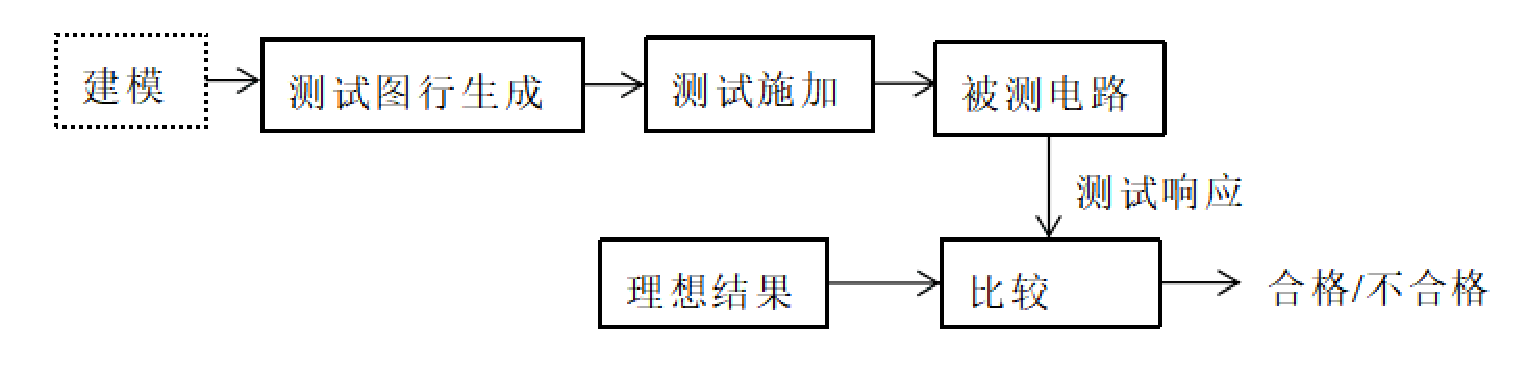
\includegraphics[height=4cm,width=16cm,angle=0,scale=1]{11.eps}
  \vspace*{0\baselineskip}
  \caption{电路测试分析过程}\label{11}
  \vspace{\baselineskip}
     \end{figure}


\subsection{生产测试和功能测试}
生产测试又被称为产品测试,通过对芯片进行缺陷测试或者故障测试以验证其是否符合标准。生产测试方案的制订必须考虑AET性能、测试功耗以及测试时长等影响因子。

功能测试就是对产品的功能进行测试,属于黑盒测试,主要通过检验芯片功能是否符合预期来判断芯片的质量。按照测试过程分类,功能测试可以分为测试施加、测试生成和测试结果验证。按测试生成的方法分类,功能测试可分为穷举测试、伪穷举测试、伪随机测试等。在相关文献\cite{19}中,总结了各类测试方法的特征以及相关术语包括(1)穷举测试、(2)伪穷举测试\cite{20}、(3) 伪随机测试\cite{21}、(4)确定性测试、(5)测试施加\cite{22,23}。

\subsection{可测性设计}

在芯片测试过程中,测试图形生成冗长且困难,于是可测性设计方法就得以发展,其主要是为了解决芯片测试过程所面临的诸多问题,比如测试时长、测试功耗、测试数据量等。因此,在设计芯片的初始阶段就需要考虑如何测试的问题。可测性设计出现于上个世纪70 年代,最先提出的是通过扫描路径\cite{24}对电路进行设计,其中一个典型的应用就是IBM进行的80286研发\cite{25}。

通常有两种方法实现可测性设计。一种方法是专项技术,另一种方法是系统化技术。对于可测性设计,著名学者Bennetts给出了一个定义,给定一个集成电路,通过耗费有限时间和成本完成对其测试,并达到预期的效果,则称此电路是可测的\cite{26}。 实质上这个定义有些含糊,不同的设计者会有不同的解释。例如,关键词“成本”,也许IC制造家为了减少测试成本就会减少这方面的可靠性开支。其流程大致为:在扫描模式下,扫描链移入一个即将被施加到组合逻辑上的测试向量。在系统模式下,经过一个时钟周期,测试向量被施加到组合逻辑上,输出响应在时钟信号下进入触发器。然后扫描链在扫描模式下将组合逻辑的输出响应移出来,同时将下一个测试向量移进去,如此反复进行直至测试完毕。

\section{国内外研究现状}

数据压缩的主要目的是为了减少测试集的数据量,下图\ref{12}给出了测试压缩结构图,由图中可以看出其中包括三个部分,第一个部分是ATE(测试设备),里面存储了压缩激励,第二个部分是CUT (被测电路),第三个部分是压缩的响应。测试过程大致为先将压缩的测试激励经过解压器,还原成为测试向量,然后将已压缩的激励送入到被测芯片上,最后将经过解压器解压缩的测试激励送入被测电路进行测试,捕获电路测试响应,若实际响应与压缩响应一致,则认为此块芯片是合格的。测试激励压缩与测试响应压缩是测试数据压缩的两个部分,根据不同的场景将采取不同的压缩方法,本文所研究的激励压缩要保证压缩之后的测试向量能准确无误地被还原,属于无损压缩。

\begin{figure}[H]
  \centering
  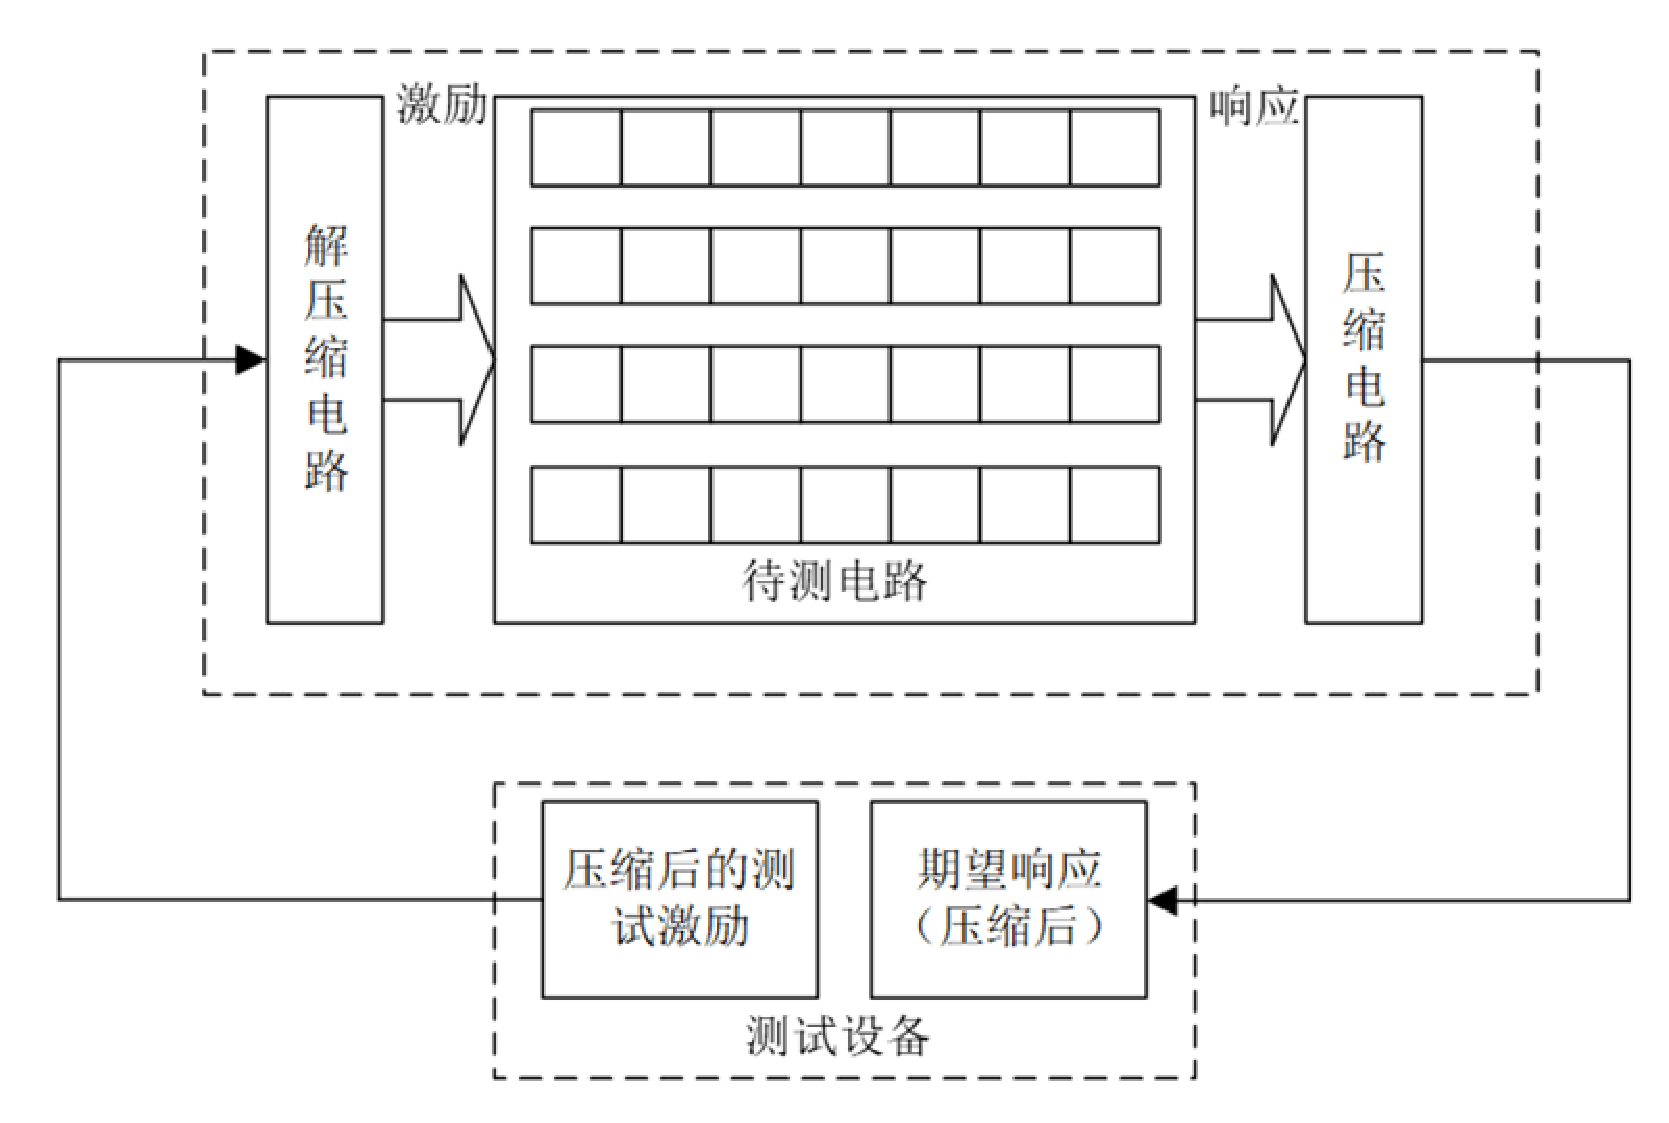
\includegraphics[height=9cm,width=15cm,angle=0,scale=1]{12.eps}
  \caption{数字电路测试压缩结构图}\label{12}
     \end{figure}

测试激励有多种压缩方式,比如编码压缩、线性扫描压缩等等。比较常用的编码有EFDR编码、FDR编码、Huffman编码以及Golomb编码。经过多年发展,近年来提出了拆分压缩这种新型压缩方法。在图像和音频信号的压缩中人们经常使用变换编码的方法,变换编码不是直接对原数据进行压缩,而是将数据以另外一种便于压缩的方式展现出来,通俗地说就是使用一种特殊的码字替换原码字,从而提高压缩率。视频压缩或者音频压缩可以将一些能量较小的数据丢弃,将其转化成为易于压缩的数据,这类压缩方法属于有损压缩。目前,测试激励压缩技术按测试数据存放的位置可以分为两类:内建自测试\cite{27,28}和测试数据压缩。

(1)内建自测试\cite{29}

内建自测试是为了快速地对集成电路进行诊断与测试,为了实现这一功能,一种合适的方式就是将测试规定为一种系统功能。

内建自测试由内建测试(built-in test ,BIT)和自测试(self-test)这两个部分组成。 BIST 是电路(芯片、板或者整机)测试自身的能力。自测试往往不是由硬件实现的,而基于软件实现的,完全基于软件的方式满足集成电路系统级别的要求,会产生诸多缺点,比如降低测试诊断分辨率、延长开发周期与时间、消耗大量的开发成本等等。

内建自测试,是一种使用器件的部分电路来测试器件本身的设计技术,它可以测试功能、结构,但不能测试参数。现在,BIST 技术主要分两种:在线(On-line)\cite{30}和离线(Off-line)。在线,进一步可分为并发在线(Concurrent on-line)和非并发在线(Noconcurrent on-line);离线,进一步可分为功能离线(Functional off-line)和结构离线(Structural on-line)。

在线 BIST,是在能够完成所需要求的情况下进行的。并发在线测试能按照所需要求完成,和其他操作同时进行,这种测试通常用编码技术或复制、比较技术以及线性反馈移位寄存器\cite{31,32}的技术来完成;非并发在线,是指能按照所需要求来完成空闲状态,也叫做后台操作,这种测试通常用软件程序来完成。在线测试是指由其他能够按照要求完成的操作,因此,在线测试能检测实时错误。

离线 BIST\cite{33}是指不能够完成所需要求的情况下进行的,通常使用输出响应分析器和测试向量生成器来完成。功能离线是根据被测器件有什么作用来测试的;结构离线是根据被测器件结构的类型来测试的。由于离线测试没有按照所需要求来完成操作,因此离线测试不能检测实时错误\cite{34}。

BIST 电路一般是由测试图形生成激励、被测电路、数据压缩的电路、进行比较分析的电路、存储理想结果的电路(ROM)和进行自测试控制电路组成,一般结构如图\ref{13}所示。

\begin{figure}[H]
  \centering
  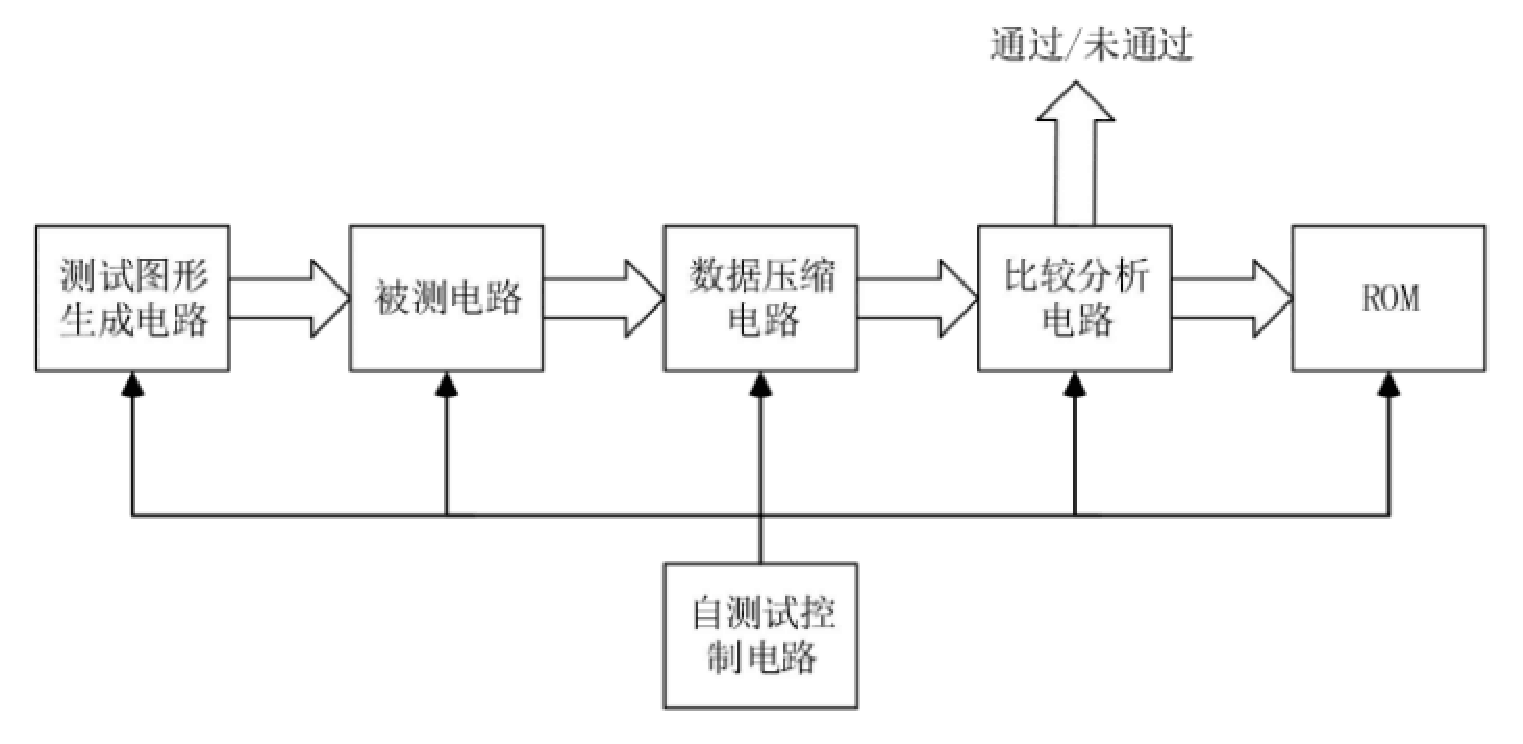
\includegraphics[height=6cm,width=14cm,angle=0,scale=1]{13.eps}
  \caption{内建自测试一般结构}\label{13}
     \end{figure}

推崇大力发展内建自测试主要分为四个目的,第一:为了解决芯片复杂度的问题。当芯片复杂度大大提升时,简单地对测试难集进行拆分是不可能的,并且使用传统化技术解决相对复杂的测试问题相当困难。BIST提供了层次化的解决方法,通过自顶向下的方式对芯片进行测试,同时为了更好地检测一块芯片,判断芯片是否存在质量问题,BIST提供了对加载原件的有效测试,减少了系统级别测试的压力。第二:解决了芯片质量低下的问题。评价芯片质量是一件复杂的任务,首先发生故障的种类不仅取决于系统、芯片,芯片的制造工艺也是不可忽略的因素。通常情况下会将芯片质量定义一个考量标准,比如将芯片的拒收率控制在十万分之1,或者将测试成本控制在一定的范围内。第三:解决了BIST 经济效益的问题。是否采用BIST方案对芯片进行设计,在生产芯片的初始阶段就是一个需要考量的问题。如果是从芯片的层面考虑,使用BIST方案不会节约较多的测试成本,但是BIST往往作用于芯片生产流程的整个生命周期,因此可以带来极为可观的收益。第四:为了解决测试应用问题。近年来,印制板测试主要基于在线测试,在线测试无法首先系统级诊断,只在板从系统拆解之后才是有效的。其次,BIST 为了解决相关测试问题提出了相关优秀的解决方法,比如,在内建自测试时,能够对整机进行测试包括芯片、零件等而避免了昂贵的外设代价,其次对于硬件板和芯片的离线测试,可以使用在系统级别测试。

BIST 的测试向量生成技术可以分为三类:穷举/伪穷举测试法;伪随机测试法;确定性测试法。内建自测是当前广泛应用的可测试性设计方法。其主要思想是测试的向量是由自身获取,不依赖于外部输入\cite{35}。

(2)测试数据压缩

在测试数据压缩方面,国外的起步较早,在1998 年,Jas 和 Touba 提出一种基于码字0编码的编码方案\cite{39},其以较短的固定码字替换较长的0码字串。在 2001 年,Lorse和Sam等人提出来一种基于 Golomb 代码的新的解压缩架构,这种全新的测试压缩方法在编码片上系统中运用广泛,通过使用单个自动测试仪I/O通道驱动片上系统中的多个核,此种解压缩架构又被称为交织解压缩架构\cite{40}。2013年,相关学着基于典型测试序列中0码字的运行分布,提出来一种可变长度的编码方式,并将其称为FDR编码
\cite{41},FDR编码是一种用于对连续0游程编码的方法,若测试集中的1码字较多,会影响压缩率。Maleh 和 Abaji 在FDR编码的基础上加以完善,提出了EFDR\cite{42}的编码方式,此种编码不仅可以对0游程编码,也适用于对1游程编码。随后Usha S. Mehta 和 Kankar S为了在游程编码的基础上进一步提高压缩率,提出了一 种 名 为 Hamming Distance Based Reordering 和 Columnwise Bit Stuffing with Difference Vector (HDR-CBS-DV)的新方案\cite{43}。同时Dasgupta 伊利诺伊大学相关研究人员提出了一种伊利诺伊扫描结构\cite{44}。文献\cite{45}提出了一种新的 LFSR 重播技术,该技术利用电路内部网络的响应作为改变 LFSR 状态的控制信号;文献\cite{46}提出了一种新颖的压缩方法和低成本的解压缩架构,它将基于符号和基于线性的技术的优势结合在一个统一的多核 SoC 解决方案中;为了减少测试响应数据,文献\cite{47}提出了一种新的测试响应压缩方案,称为选择性测试响应集;

国内在数据压缩领域起步较晚,但是也有相关研究成果被提出。文献\cite{48}提出了一种测试数据压缩方法,它结合了基于字典的压缩和基于位掩码的压缩的优点,是一种基于非固定的索引,它使用较短的索引来表示具有较高出现频率的切片,而使用较长的索引来表示具有较低出现频率的切片,然后采用有效的位掩码和基于最大度的 Clique 分区算法来创建尽可能多的兼容切片,文中还提出了一种新的可变前缀双游程代码来压缩不兼容的切片来减少测试数据量;文献\cite{49}提出了一种考虑模式信息维度的基于游程的压缩方法;文献\cite{50} 提出了一种选择性模式压缩方案,可以在基于扫描的测试期间,有最小的测试功率和测试数据量;文献\cite{51}提出了一种二维(空间/时间)压缩技术,可以减少测试数据量并测试知识产权内核扫描测试的应用时间。

通常而言测试数据压缩框架如图1.4所示,ATE上存储了所有的测试数据,购买自动测试仪价格昂贵,因此往往会将测试数据进行压缩节约成本\cite{36,37,38},因此在原有的基础上必须设计解压缩电路,将测试数据还原,其框架图流程图如下图\ref{14}所示。

\begin{figure}[H]
  \centering
  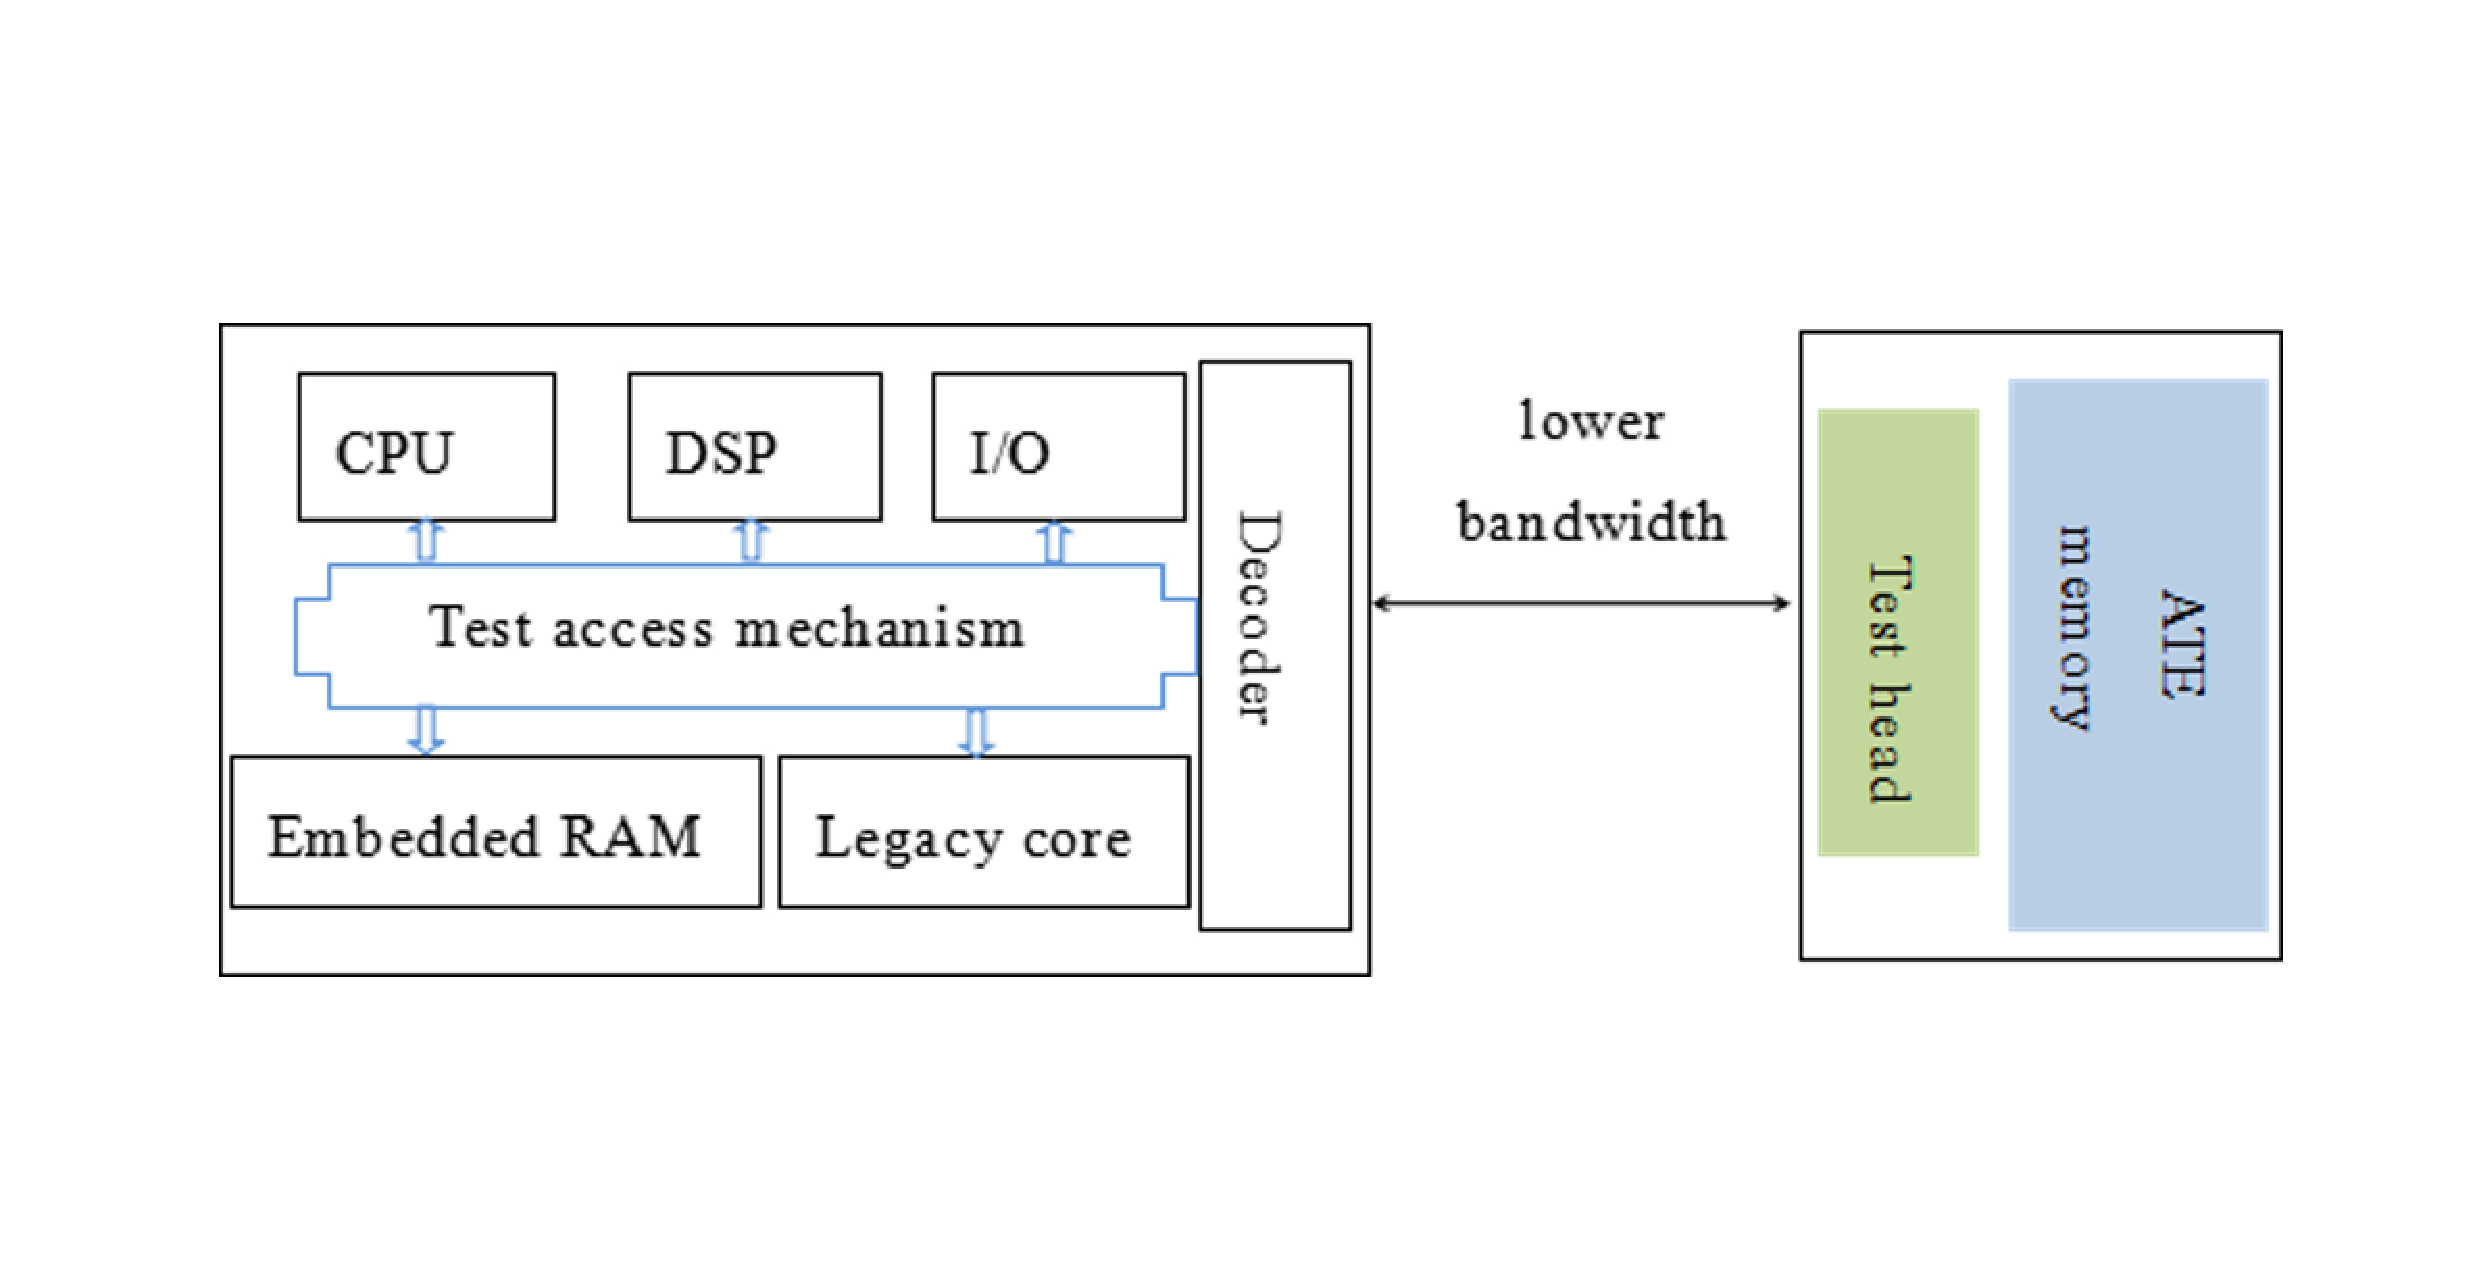
\includegraphics[height=8cm,width=16cm,angle=0,scale=1]{14.eps}
  \caption{TRP框架图}\label{14}
     \end{figure}

\section{本文主要工作及组织结构}

本文在拆分压缩的基础上,主要针对基向量的生成方式进行了研究。由于主分量集是由基向量确定的,因此基向量选取的好坏将导致最终压缩率的高低。生成主分量集的方法有哈达码变换、K-L 变换、离散余弦变换等,本文在拆分压缩的基础上,提出来两种基向量生成算法,一种是将测试集预填充后,以列向量间欧几里得距离最大为原则选取基向量,第二种是使用聚类算法生成实验所需的基向量。同时本文还将聚类算法与位翻转算法进行结合进一步提高压缩率。这三种方法针对压缩率都达到了较好效果。

文本总共分为五个章节阐述自己的工作:

第一章是绪论部分,首先介绍了集成电路发展的背景以及电路测试的相关先修知识,其次就国内外研究现状进行分析最后总结本文的组织结构。

第二章主要就常用的压缩方法做了详细地介绍。第一部分讲解了编码压缩技术,包括游程编码、字典编码以及统计编码。第二部分就基线性解压缩和广播扫描两种非编码压缩方法做出了相应的分析与阐述,最后介绍了拆分压缩技术和哈达码变换,并对哈达码变换的优缺点进行了分析。

第三章重点介绍了使用预填充策略处理数据集的方法,包括填充规则、基向量的选取等步骤。

第四章详细介绍了相关聚类算法以及如何将聚类算法应用于测试电路压缩的具体步骤。同时本章进行了大量的实验用于验证此方法的有效性,并通过动态选取基向量数,较好地反映出压缩率与基向量个数之间的线性关系。

第五章介绍了位翻转算法的相关概念与计算流程,并将kmeans++算法结合位翻转算法进一步提高压缩率。

最后总结全文,并对该研究工作中的问题进行了展望。
